\subsection{Static Analysis}
The first step is understanding the structure and behaviour of the application. As the source code is not publicly available we must be satisfied with the second-best option which is decompilation. There is a range of tools to decompile an android application, the one we will use is \href{https://github.com/skylot/jadx}{jadx}\footnote{\href{https://github.com/skylot/jadx}{https://github.com/skylot/jadx}}. The newest apk is retrieved from \href{https://apkpure.com/guloggratis/dk.guloggratis}{apkpure}\footnote{\href{https://apkpure.com/guloggratis/dk.guloggratis}{https://apkpure.com/guloggratis/dk.guloggratis} - at the time of the analysis the newst version was 2.5.4, but version 5.0.1 was released the 25th of November}. The apk is then decompiled using jadx resulting in two folders, one with source code and the other with resources. The source code folder contains all the logic of the application together with the wide range of libraries used. While the resource folder contains static resources such as images, xml configuration files, hardcoded strings, etc.

It is not easy to identify which parts should be investigated in such a decompilation. Firstly a manual search was conducted searching for keywords. The keywords use of cryptographic algorithms, secrets, keys or passwords. Nothing interesting resulted from the manual search. Then the source code  was looked at to understand the flow and structure. It was clear that no apparent use of obfuscation is used. The code is both easy to read and understand. An example can be seen on figure \ref{fig:ggapplication-properties} 

\begin{figure}[htbp]
    \centering
    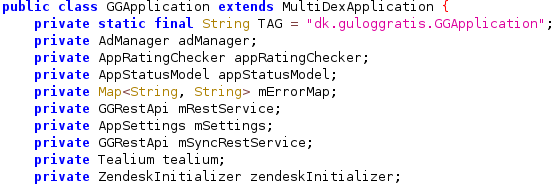
\includegraphics[width=1\columnwidth]{../static-analysis/pictures/GGApplication_properties.png}
    \caption{ORL example images}
    \label{fig:ggapplication-properties}
\end{figure}

This is a snippet from the start of a class, that initializes services and makes them available across the application. There is neither use of name obfuscation nor string encryption. As a consequence it is easy for an adversary to understand the code flow and in this case identify some of the services used in the application.

To easen the static analysis \href{https://github.com/MobSF/Mobile-Security-Framework-MobSF}{MobSF}\footnote{\href{https://github.com/MobSF/Mobile-Security-Framework-MobSF}{https://github.com/MobSF/Mobile-Security-Framework-MobSF}} is used to identify known flaws and vulnerabilities. MobSF indicates the application has a security score of 35/100, which might indicate that there is some vulnerabilities. Looking at the report there several configurations, that is tagged as medium or high Severity. One is the allowance of application data backup. This is a flag that defaults to true. If sensitive data is stored this should be considered actively set to false. In the code analysis it shows there is a massive amount of logging. Some of this logging can be seen in a search on figure \ref{fig:log-payments}.

\begin{figure}[htbp]
    \centering
    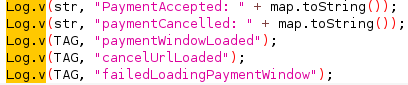
\includegraphics[width=1\columnwidth]{../static-analysis/pictures/log_payments.png}
    \caption{Search of log statements}
    \label{fig:log-payments}
\end{figure}

These log statements are called in callback functions from an external library containing dibs logic. Dibs is basically NETS which is used to perform payments. These log statements can contain sensitive payment information and should not be included in a release build. A way to avoid this is using \href{https://github.com/JakeWharton/timber}{timber}\footnote{\href{https://github.com/JakeWharton/timber}{https://github.com/JakeWharton/timber}}. Timber is a wrapper that enables the possibility of only enabling log statements in debug builds. Timber is used for some parts of the application but neglected in other parts.    

Another potential flaw is aswell found in the used dibs library. The library utilizes a webViewClient which is embedding a browser in the application. The code can be seen on figure \ref{fig:dibs-webview}. The code enables javascript in the embedded browser and adds an interface to Java code. This is a known vulnerability to all android sdk versions below 17\cite{avg-webview-explot}. Since the application has a minimum sdk version of 21 and above, this is not an issue.  

\begin{figure}[htbp]
    \centering
    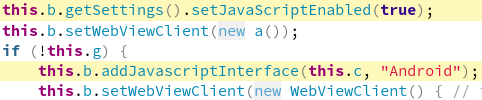
\includegraphics[width=1\columnwidth]{../static-analysis/pictures/dibs-javascript.png}
    \caption{Dibs library embedded webview}
    \label{fig:dibs-webview}
\end{figure}

Another webview vulnerability is aswell seen in a used library. This can be seen on figure \ref{fig:zendesk-webview}. Here the webview is set to debuggable. This means it's possible to attach an debugger and see/control the execution of the webview.    

\begin{figure}[htbp]
    \centering
    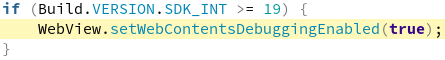
\includegraphics[width=1\columnwidth]{../static-analysis/pictures/zendesk-webview.png}
    \caption{Zendesk library embedded webview}
    \label{fig:zendesk-webview}
\end{figure}

The report from MobSF aswell display the use of SSL pinning. This can be seen on figure \ref{fig:ssl-pinning} and will be analyzed later in the attempt of a man-in-the-middle attack. 

\begin{figure}[htbp]
    \centering
    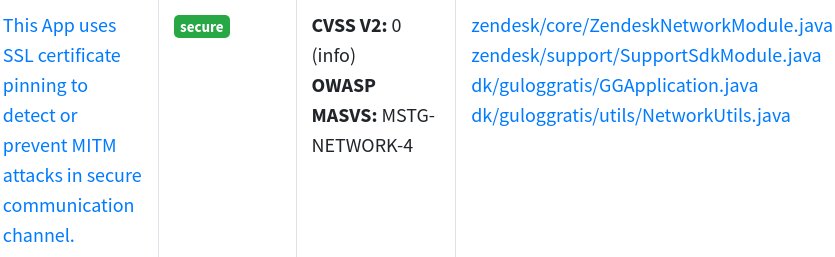
\includegraphics[width=1\columnwidth]{../static-analysis/pictures/ssl-pinning.png}
    \caption{Usage of ssl-pinning}
    \label{fig:ssl-pinning}
\end{figure}

\subsection{Dynamic Analysis}
A dynamic analysis was performed using MobSF. A emulator with sdk version 29 is spawned locally using \href{https://www.genymotion.com/}{genymotion}\footnote{\href{https://www.genymotion.com/}{https://www.genymotion.com/}}. MobSF then installs an instrumented app with configurations of our choice. The defaults are selected which includes: installing root ca, setup https proxy, certificate pinning bypass, etc. Then some execution flows are performed on the device and a report is generated. It's then possible to see various information of the execution. The network traffic can be seen. These requests are sent to \href{https://portswigger.net/burp}{Burp Suite}\footnote{\href{https://portswigger.net/burp}{https://portswigger.net/burp}}, and will be analyzed in the next section. The hostnames and their geolocation can aswell be seen together with trackers. It is also possible to see log statements. A example can be seen on figure \ref{fig:log-login-request}. It shows that urls together with query parameters are logged.  

\begin{figure}[htbp]
    \centering
    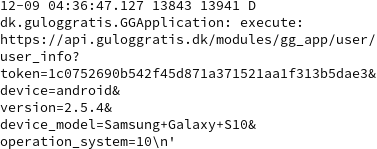
\includegraphics[width=1\columnwidth]{../static-analysis/pictures/log-login-request.png}
    \caption{Logging HTTP traffic}
    \label{fig:log-login-request}
\end{figure}

The generated report also shows the local files stored in the applications own data directory. An example is a XML file stored in SharedPreferences. A snippet of the file can be seen on figure \ref{fig:gull-prefs-xml}. It is seen that the token stored is the one used in HTTP requests.  

\begin{figure}[htbp]
    \centering
    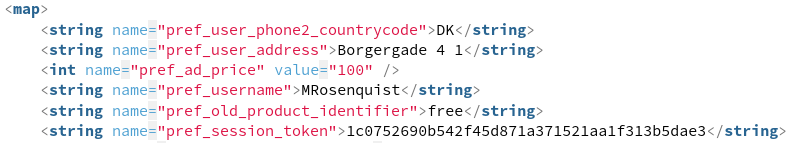
\includegraphics[width=1\columnwidth]{../static-analysis/pictures/gull-prefs-xml.png}
    \caption{Part of xml preference file}
    \label{fig:gull-prefs-xml}
\end{figure}